%%
%% This is file `sample-sigconf.tex',
%% generated with the docstrip utility.
%%
%% The original source files were:
%%
%% samples.dtx  (with options: `all,proceedings,bibtex,sigconf')
%%
%% IMPORTANT NOTICE:
%%
%% For the copyright see the source file.
%%
%% Any modified versions of this file must be renamed
%% with new filenames distinct from sample-sigconf.tex.
%%
%% For distribution of the original source see the terms
%% for copying and modification in the file samples.dtx.
%%
%% This generated file may be distributed as long as the
%% original source files, as listed above, are part of the
%% same distribution. (The sources need not necessarily be
%% in the same archive or directory.)
%%
%%
%% Commands for TeXCount
%TC:macro \cite [option:text,text]
%TC:macro \citep [option:text,text]
%TC:macro \citet [option:text,text]
%TC:envir table 0 1
%TC:envir table* 0 1
%TC:envir tabular [ignore] word
%TC:envir displaymath 0 word
%TC:envir math 0 word
%TC:envir comment 0 0
%%
%% The first command in your LaTeX source must be the \documentclass
%% command.
%%
%% For submission and review of your manuscript please change the
%% command to \documentclass[manuscript, screen, review]{acmart}.
%%
%% When submitting camera ready or to TAPS, please change the command
%% to \documentclass[sigconf]{acmart} or whichever template is required
%% for your publication.
%%
%%
\documentclass[sigconf]{acmart}
%%
%% \BibTeX command to typeset BibTeX logo in the docs
\AtBeginDocument{%
  \providecommand\BibTeX{{%
    Bib\TeX}}}

%% Additional packages for subfigures
\usepackage{subcaption}
\usepackage{algorithm}
\usepackage{algorithmic}


%%
%% end of the preamble, start of the body of the document source.
\begin{document}

%%
%% The "title" command has an optional parameter,
%% allowing the author to define a "short title" to be used in page headers.
\title{3D Spatial Scene Description for and Guidance for Visually Impaired People}


\author{Lukas Ederer}
\email{ederer0@hm.edu}
\affiliation{
  \institution{University of Applied Sciences Munich}
  \city{Munich}
  \state{Bavaria}
  \country{Germany}
}

\author{Jan Duchscherer}
\email{j.duchscherer@hm.edu}
\affiliation{
  \institution{University of Applied Sciences Munich}
  \city{Munich}
  \state{Bavaria}
  \country{Germany}
}

%%
%% The abstract is a short summary of the work to be presented in the
%% article.
\begin{abstract}

\end{abstract}

%%
%% Keywords. The author(s) should pick words that accurately describe
%% the work being presented. Separate the keywords with commas.
\keywords{3D Spatial Understanding, Assistive Technology, Visually Impaired, Gemini,
Large Language Models (LLMs), Interactive Audio Guidance, Semantic Segmentation, Mobile Navigation,
Human-Computer Interaction (HCI), Obstacle Avoidance}

%% A "teaser" image appears between the author and affiliation
%% information and the body of the document, and typically spans the
%% page.
\begin{teaserfigure}
  \begin{subfigure}{0.48\textwidth}
    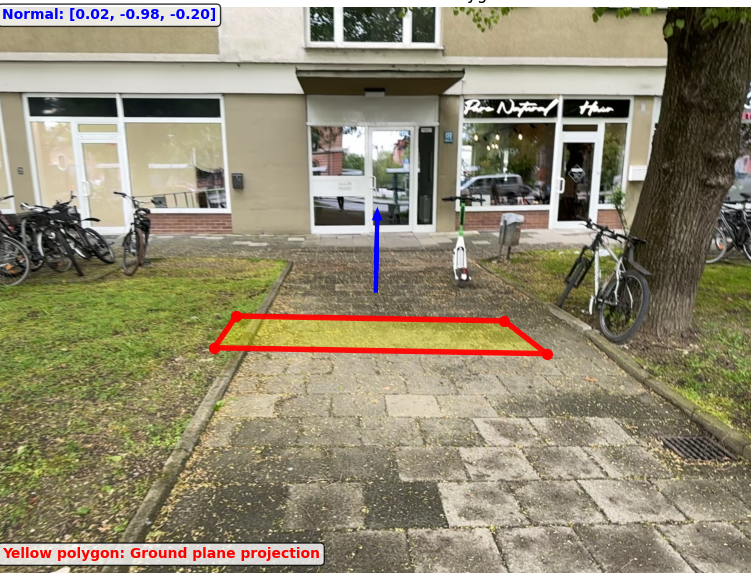
\includegraphics[width=\textwidth]{figures/ransac.png}
    \caption{RANSAC ground plane detection for height estimation.}
    \label{fig:teaser:ransac}
  \end{subfigure}
  \hfill
  \begin{subfigure}{0.48\textwidth}
    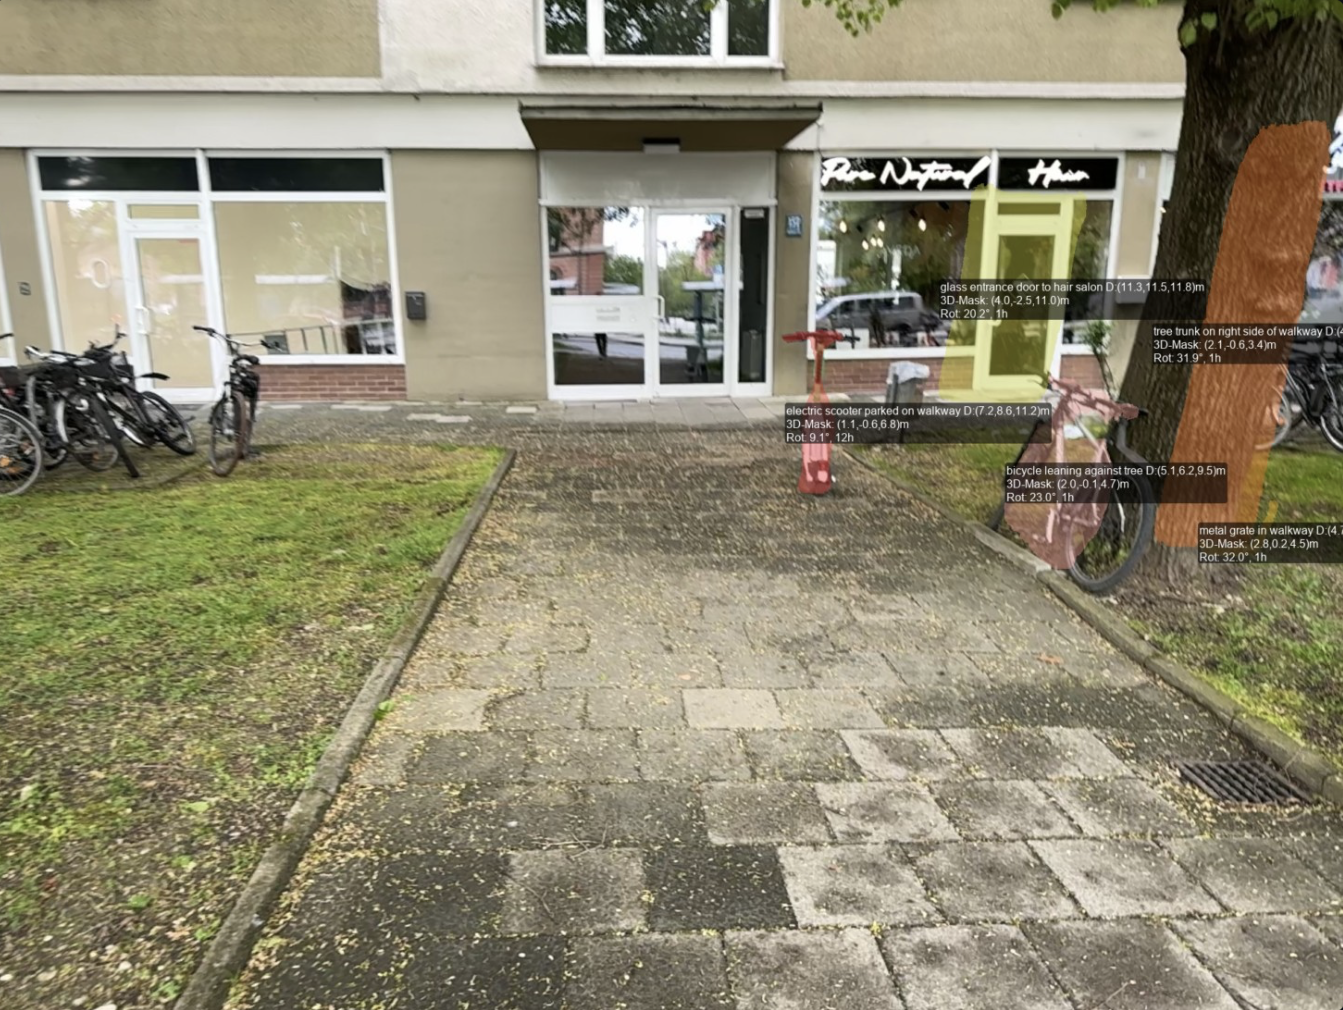
\includegraphics[width=\textwidth]{figures/path_desc.png}
    \caption{Segmentations of objects relevant for navigating to the entrance of the hair salon.}
    \label{fig:teaser:path}
  \end{subfigure}
  \caption{Overview of our 3D spatial understanding system: (a) Ground plane detection using RANSAC algorithm with object detection and spatial relationships, and (b) Interactive guidance system providing spatial descriptions and navigation assistance.}
  \label{fig:teaser}
\end{teaserfigure}


\maketitle

\section{Introduction}
It is not always easy to navigate a city environment, especially for people with visual impairments.
Often times there are obstacles in the way that can be hard to detect, or there is no clear path to follow.
Using commen navigation systems or apps that use 2D data or gps is not always sufficient to provide the necessary information for navigation.
Often times it is necessary to have a 3D understanding of the environment in order to navigate around safely.
This is where the idea of a 3D spatial scene description system comes into play.
The goal of this project is to create a system that can help users navigate through their environment by providing spatial guidance.
The app should combine knowen VLM capabilities with 3D data to provide spatial information.
It should help the user by giving him information about the location, height and distance of objects around him.
There should also be a way of getting further navigation assistance by providing a way to ask questions about the environment.

\subsection{Research Question}
After analysing the current state of the field and the above mentioned goals, the following research question was formulated:
\begin{quote}
\textit{How can a 3D spatial scene description 
system effectively translate visual and 
depth information into guidance to 
improve navigation of blind and visually 
impaired individuals.}
\end{quote}



\section{Background}

\subsection{RANSAC}
% Content about RANSAC algorithm for ground plane detection
% - Mathematical foundations
% - Application in spatial understanding
% - Implementation details

\subsection{Depth Calculation}
% Content about depth calculation methods
% - Depth estimation techniques
% - Integration with RGB data
% - Accuracy considerations

\subsection{Gemini SDK}
% Content about Gemini SDK capabilities
% - Live API functionality
% - Structured outputs
% - Integration methods
% - Performance characteristics

\subsection{Native Capabilities of Gemini and other VLMs}
% Content about VLM capabilities for spatial understanding
% - Scene understanding capabilities
% - Spatial reasoning
% - Object detection and recognition
% - Limitations and strengths

\section{Related Work}

As discussed in previous studies~\cite{googleFinetuning2025}, spatial understanding for assistive technology is an active research area.

\subsection{Spatial Understanding Systems}

\subsubsection{SpatialBot}
SpatialBot is a VLM designed for spatial tasks, by incorporating depth images and data into its outputs.
It is trained on a hierarchy of spatial tasks, with are categorized as low, middle and high-level.
\begin{itemize}
    \item \textbf{Low-level tasks:} Direct querying of depth values from a depth map and exact information of these on set points
    \item \textbf{Middle-level tasks:} Comparing distances between objects, and calculating the relative position of objects in a scene.
    \item \textbf{High-level tasks:} Understanding spatial relationships between objects and doing things like counting objects in a scene.
\end{itemize}

It has been successfully deployed in robotic systems, where it can be used to translate spatial understanding into physical actions.
This highlights the robustness of its capabilities with would help in guidance systems, where it is important to get correct spatial information to the user.

Another feature that is highlighted in the paper is the ability to distinguish between real and printed objects by using the spatial depth information provided by the depth images.
This can also help in navigation where detecting hazards is important, with also means the system needs to be able to decide if an object is a poster or a real thread.

Internally the SpatialBot framework uses a fine-tuned VLM with a curated RGB-D dataset.
It tries to specifically address the challenge of providing consistent and accurate information for robotic systems.
As seen later in this paper, we also used a lot of the same concepts in mapping depth values and providing spatial information als seen here.\cite{SpatialBotCai2025}

\subsubsection{Video-3D LLM}
Video-3D LLM is a model that enhances Multimodal Large Language Models (MLLMs) with sophisticated 3D spatial understanding capabilities.
This tackles the challenge, that most MLLMs are only trained on 2D data with limits there capabilities in spatial reasoning.
It is treating 2D scenes as dynamic videos and incorporating 3D data into the video representation.
This allows a more accurate understanding and goes in line with the goal of using a smartphone video stream as an input for our system.

\begin{itemize}
    \item \textbf{Position-Aware Video Representation:} It is not using the traditional approach of converting 3D scenes into point clouds. Instead it directly processes video frames along with their corresponding 3D global coordinates. It does this by back-projecting pixel from the depth image and then encoding and injecting the visual features to give the option of getting spatial information.
    \item \textbf{Efficient Frame Sampling:} To handle larger video sequences, it uses a sampling strategy where it only uses the the minimum number of frames needed to get all the spatial information.
    \item \textbf{Multi-Task Generalist Model:} As a single model it can handle task like, describing objects, locating objects and answering questions about objects that require spatial reasoning.
\end{itemize}

Even though it might seem like a perfect fit for our usecase it still comes with some limitations.
For example, it is trained on indoor scenes and would probably not be able to handle outdoor scenes as well.
Its compute time for processing a video is also quite high, making it difficult to use in a real-time setting. \cite{zheng2024video3dllmlearningpositionaware}

\subsubsection{SpatialVLM}
\label{ssec:spatialvlm}

SpatialVLM~\cite{spatialvlmChen2024} by Google DeepMind is a data-synthesis and pre-training framework designed to endow generic vision-language models (VLMs) with \emph{quantitative} spatial reasoning capabilities.  It converts monocular RGB images into \emph{canonicalised}\footnote{The authors define \emph{canonicalisation} as a RANSAC-based alignment of the depth-derived point cloud to a physically meaningful world frame whose $z$-axis is normal to a detected horizontal support surface (e.g.\ floor or tabletop).} 3-D scene graphs and uses these graphs to auto-generate an internet-scale spatial VQA corpus.

\paragraph{System overview.}
The \emph{data synthesis pipeline} comprises four off-the-shelf expert models: CLIP to filter images of real world scenes, open-vocabulary detection, semantic segmentation, monocular metric depth estimation (ZoeDepth~\cite{ZoeDepthBhat2023}), and object-centric captioning.  Detected regions are lifted to a metric point cloud, canonicalised as described above, and clustered into object instances whose centroids, sizes, and pairwise Euclidean distances are computed, resulting in a spatial graph where objects are represented by vertices and relations between them are quantitative relationships. A templated question-answer generator then produces \(\sim\!2\text{billion}\) QA pairs over \(10\text{ million}\) real-world images, covering \textbf{38} qualitative and quantitative spatial relation types (e.g.\ \emph{left-of}, \emph{higher-than}, exact metric distance).

\paragraph{Generated dataset.}
The resulting VQA dataset mixes 50 \% qualitative and 50 \% quantitative questions.  \emph{One-sentence overview:} it spans fine-grained prompts such as ``\textit{How far is the blue mug behind the red plate?}'' or ``\textit{Which object is wider, the laptop or the book?}'', always answered in human-like units and rounding.

\paragraph{Downstream use.}
SpatialVLM's synthetic QA pairs were used to \emph{pre-train Googles Gemini models}, endowing them with foundational spatial reasoning capabilities that were evidentally extended to endow Gemini models with AABB and OBB detection, as well as semantic segmentation capabilities.

\paragraph{Criticism.}
While the framework captures metric distances and relative size/position, it omits \emph{relative orientations} (e.g.\ object yaw or facing direction).  Incorporating such labels—even if users rarely ask explicitly—could further enrich the learned inductive biases and enable reasoning about tasks like ``\emph{Is the chair facing the table?}'' or ``\emph{What's the yaw between the red car and the parked scooter?}''.

\subsection{Key Concepts and Limitations}
% Content about relevant concepts and limitations from existing work
% - Common approaches in spatial understanding
% - Identified gaps in current solutions
% - Challenges in real-world deployment
% - Opportunities for improvement

\section{Concept}

\subsection{System Architecture}
% Content about system architecture (Jan)
% - Sequence diagram to explain different use cases/data flow in the application
% - How we use Live API, Gemini Pro, etc.
% - Overall system design and components

\subsection{Core Features}

\subsubsection{Full Scene Description}
% Content about comprehensive scene understanding and description
% - Scene analysis approach
% - Information extraction methods
% - Description generation

\subsubsection{Spatial Information on Individual Objects}
% Content about object-level spatial processing
% - Rotation: Object orientation detection
% - Depth: Distance measurements
% - 3D Points: Spatial coordinate calculation
% - Erosion: Image processing techniques
% - MAD: Median Absolute Deviation calculations

\subsection{Advanced Spatial Processing}

\subsubsection{Caching of Detections}
% Content about performance optimization through caching
% - Detection caching strategy
% - Performance improvements
% - Memory management

\subsubsection{SE(3) Transformations}
% Content about spatial transformations
% - SE(3) into Ego Frame: Transformation to ego-centric coordinates
% - SE(3) for Frame Change: Model context transformation
% - Mathematical foundations

\subsubsection{Height Information with RANSAC}
% Content about ground plane detection
% - RANSAC implementation for ground plane detection
% - Height calculation methods
% - Accuracy and robustness

\subsection{Path Description}
% Content about navigation guidance generation
% - Path analysis and description
% - Navigation instruction generation
% - User interaction design

\subsection{Path Description}

\section{Evaluation}

\subsection{Testing Methodology}
In order to evaluate the functionality of the application a series of tests were conducted.
To assure that the results are consisted and comparable, the same setup, prompt, input data was used for each run.
There was also a focus of using the same scenes and objects for each test to make it easier to compare results and find outliers.
The input and some of the results can be found in the appendix.
For classification and segmentation the Gemini Pro 2.5 model that was released on the 16th of June 2025 was used.

Throughout the later development of the application the gemini-2.5-pro-preview-05-06 model was used.
With this configuration we were able to get good results and valid outputs.
Since the release of further versions the quality as decreased significantly.
Especially the segmentation quality and validity of the structured json outputs.
The evaluation is still using the newest model though, since it is the most recent version and therefore a current representation of the apps capabilities.
Additionally, it is not possible to use the older model anymore, since it now redirects to the newest version \cite{googleGemini25Pro2025}. 

\subsection{Tool Usage}
A very important aspect is the correct use of the function calling.
When the live api detects that a user might want a more complex operation, like the distance to a specific object, or more complex navigation instructions, it will call a function that triggers the needed process.
In order to evaluate the tool usage, a series of tests were conducted, where the live api needed to use function calling to conduct an answer.
throughout the tests multiple values for temperature, top k and top p were used to see the effect on the tool usage.
There it was found, that there was no significant impact of these values in situations in which the model was not able to correctly use function calling.
Currently the values are set to temperature 0.1, top k 64 and top p 0.9.
Is seems like regardless of the values used, there are constellations in which the model is not able to function correctly.
A example of this can be seen in the following screenshot \ref{fig:tool_usage}.
It is not possible to directly identify the reason for this, as it is also unclear how the model uses the temperature, top k and top p values.
Though it can be suspected that a better system prompt and a more detailed function description could help in these cases.
Additionally, it is also possible to force function calling which could be tried as a normal conversation at a temperature of 0.1 as currently used is not working anyway.

\begin{figure}[H]
\centering
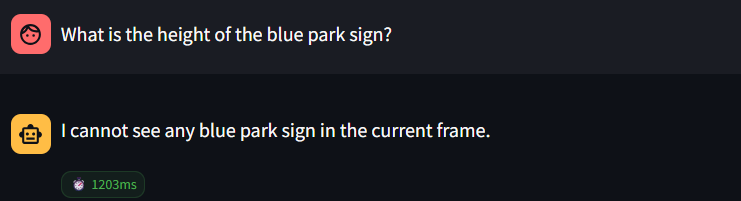
\includegraphics[width=0.4\textwidth]{figures/tool_usage.png}
\caption{Tool usage results for the same scene in multiple runs.}
\Description{A screenshot showing how tool use was not working in a specific run}
\label{fig:tool_usage}
\end{figure}


\subsection{Distance Calculation}

In order to evaluate the distance calculation in relation to the segmentation and a series of tests were conducted using the Gemini Pro model.
Because there is no labelled dataset available for this task it was not possible to create a ground truth for specific objects.
Instead, the distance calculation was evaluated by comparing the results of multiple runs against each other.
This way it is possible to see the run to run variance of the calculation and get a feel for the accuracy and consistency.
In order to create a accurate comparison the same picture, depth map and prompt was used in each run.
All of the runs did a new detection of objects in the scene. 
This way it is also possible to see the variance in object detection.
There it could be seen that a full segmentation of an entire scene reaching the limits of the model, with can result in defect or wrong json outputs.
The results show that objects that are about 4 to 5 meters away from the camera can be detected with consisted distance values \ref{fig:distance_calculation}.
Only on objects that are further away larger errors can be measured.
At this range another issue can also be seen in the lidar sensor which is only rated for about 10 meters on the iPhone 16 Pro \cite{applelidar2025}.

\begin{figure}[H]
\centering
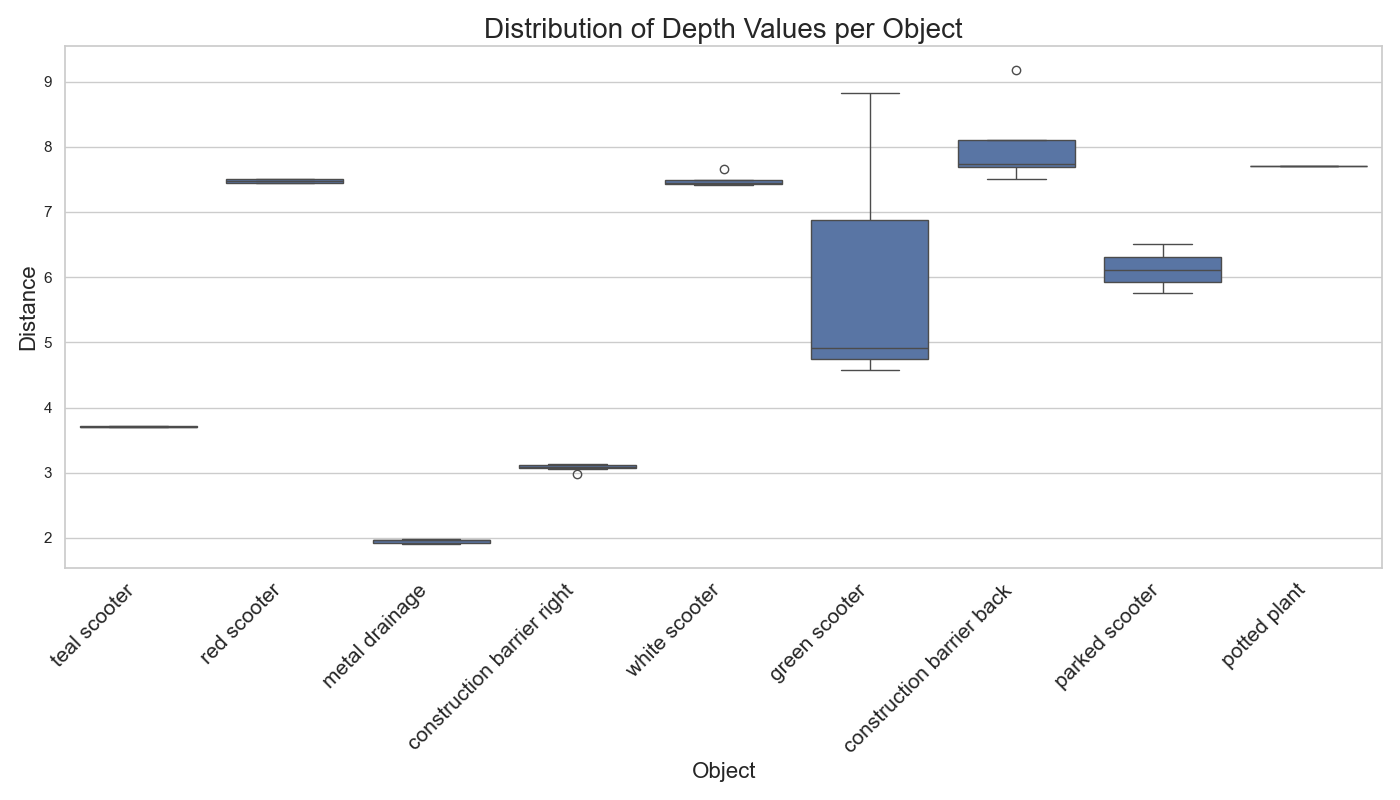
\includegraphics[width=0.4\textwidth]{figures/depth_distribution.png}
\caption{Distance calculation results for the same scene in multiple runs.}
\Description{A chart or graph showing the distribution of distance calculations across multiple test runs for the same scene, illustrating the variance and consistency in depth estimation results.}
\label{fig:distance_calculation}
\end{figure}

\subsection{Segmentation Quality}

Now that we have a visual representation of the average distance we should also take a look at the quality of the segmentation masks that were generated in each run.
The masks were ranked based on the following criteria:
\begin{itemize}
    \item \textbf{Good:} The mask is accurate and covers the object completely.
    \item \textbf{Too big:} The mask is larger than the object, but still covers it.
    \item \textbf{Too little:} The mask is smaller than the object, but still covers a significant part of it.
    \item \textbf{Wrong:} The mask does not cover the object at all or covers the wrong object.
\end{itemize}

As you can see in the Table \ref{tab:segmentation_quality} the segmentation masks vary in quality between different objects but not so much between runs.
For example, the bike was segmented correctly in every run, with one being off by a little bit.
Meanwhile the trash can was not detected at all even though it was clearly visible on screen and could be a potential hazard for the user.
The scooter was always detected in the right position, but the small size of the handlebar made it difficult for the model to segment it correctly.
This is not a problem in this case, since the depth estimation can still work as intended with the segmentation mask not being perfect.
As already mentioned, the tests where conducted on the new Gemini Pro 2.5 model, which could harm quality.

\begin{table}[H]
\centering
\resizebox{\columnwidth}{!}{%
\begin{tabular}{|l|cccc|c|}
\hline
 & \multicolumn{4}{c|}{Segmentation quality} & \\
\cline{2-5}
 & High Fidelity & Oversegmentation & Undersegmentation & Segmentation Failure & Sum of tries \\
\hline
Teal Scooter &2 & 1& 1 & 1 & 5 \\
Trash can & & & & 5 & 5 \\
Bike & 4 & 1 & & & 5 \\
\hline
\end{tabular}%
}
\caption{Segmentation quality of different objects throughout different runs.}
\label{tab:segmentation_quality}
\end{table}

\section{Discussion}


\subsection{Potential future work}


\subsection{Limitations}

\section{Conclusion}

As already stated in the introduction, the goal of this project was to crate a system that can help users navigate through their environment by providing spatial guidance.
In this work we have shown a 3D spatial scene description system that leverages Gemini VLM to translate visual and depth information into a way to explane the environment to the user.
With the solution crated it is possible to get the location or height of objects, as well as further orientation assistance.

Returning to the original research question, we can conclude that the work in this field is still in its infancy and even thoughout the time of working on this project there were multible relesases that changed our apprach.
None of the models that are used in this project were available at the start of this research project.
This also shows that there is still work to do and that the field is still evolving with could potentialy outdate this solution in the following months.
Still the results showen in the evaluation section reveal that it is possible to get accurate and consistend navigation and spatial guidance information by using the Gemini Pro Model and Gemini Live API.
This way it is not only possible to get accurate information, but the live api also allows for a easy to implement way of creating a real time conversation with the user.

\subsection{Future Work}

As showen in the discussion section, there are still limitations of the current solution hat can be fixed in the future.
The two most important ones are Model and Performance enhancements and System integration:

\begin{itemize}
    \item \textbf{Model and Performance Enhancements:} One aspekt in order to improve the performance would be to futher use example in- and outputs to get better json quality and results. Additionally, add ensembling techniques to the system could also help. This would mean to use bach requests in order to get multiple results for the same input and then use a voting system to decide witch result to pick. Another would be to seperate the segementation and formatting in two different models. The one that does the segementation could use a higher temperature while the one for formatting would use a lower temperature. This way the segmentation model could be more creative in its outputs, while the formatting model would be more strict and consistent in its outputs. Another idea would be to introduce a confidence score for the segementation masks, which would allow the user to see how confident the model is in its segmentation. This could help the user to understand the quality of the segmentation and make better decisions based on that.
    \item \textbf{System Integration:} Another aspect that can be enhanced is the implementation of the system in a real world scenario. This would include the integration of the system into a moble app with would come with its own challenges. For exampele, the system would need to use Websocket connections to the Gemini Live API in order to provice real time conversations.
\end{itemize}


\section{Team}

% Content about team contributions
% - Table showing who has done what (maybe timeline/Gantt chart)
% - Individual contributions and responsibilities:
%   - Lukas: Abstract, Introduction, Related Work (SpatialBot, VideoLLM3D), Evaluation
%   - Jan: Concept, Related Work (SpatialVLM), Limitations
% - Collaborative aspects of the project
% - Timeline of major milestones

\begin{table}[h]
\centering
\begin{tabular}{|l|l|l|}
\hline
\textbf{Team Member} & \textbf{Primary Responsibilities} & \textbf{Secondary Contributions} \\
\hline
Lukas Ederer & Abstract, Introduction, Evaluation & Related Work (SpatialBot, VideoLLM3D) \\
\hline
Jan Duchscherer & Concept, Limitations & Related Work (SpatialVLM) \\
\hline
\end{tabular}
\caption{Team member contributions and responsibilities}
\label{tab:team}
\end{table}

\begin{acks}
To Tobias, for his support and guidance throughout this project.
\end{acks}

%%
%% The next two lines define the bibliography style to be used, and
%% the bibliography file.
\bibliographystyle{ACM-Reference-Format}
\bibliography{sample-base}

\appendix

\section{Technical Details}

\subsection{Actor Pattern Implementation}
% Content about actor pattern implementation
% - Design principles and architecture
% - Implementation details
% - Benefits for the spatial understanding system
% - Code examples and patterns used

\subsection{Gemini Best Practices}
% Content about Gemini best practices
% - Optimal prompt engineering techniques
% - Parameter tuning guidelines
% - Performance optimization strategies
% - Error handling and robustness considerations

\subsection{Mathematical Foundations}
% Content about mathematical foundations
% - SE(3) transformations
% - RANSAC algorithm details
% - Depth calculation formulas
% - Spatial coordinate systems

\subsection{System Architecture Diagrams}
% Content about system diagrams
% - Sequence diagrams for different use cases
% - Data flow diagrams
% - Component interaction diagrams
% - API integration patterns


\appendix

\end{document}
\endinput
